% ============================================================================
% CHAPTER 3 --- PRNet: PAPR REDUCTION VIA DEEP AUTOENCODER
% ============================================================================
\chapter{PRNet: PAPR Reduction via Deep Autoencoder}
\label{ch:prnet}

\begin{motivation}[From Searching to Learning]
    Classical SLM carries two practical costs: (i)~computational overhead --- $U$ full IFFT operations and $U$ PAPR comparisons for every single OFDM symbol, and (ii)~side information --- $\lceil\log_2 U\rceil$ bits that must reach the receiver without error, or the entire symbol is lost.

    What if, instead of \emph{searching} over a fixed set of phase sequences, we could \emph{learn} a mapping that inherently produces low-PAPR signals? A mapping so deeply integrated into the transmitter that it needs no search, no candidate comparison, and no side information at all?

    This is exactly what Kim et al.\ (2017) proposed with the \textbf{PAPR Reduction Network (PRNet)} --- the first work to apply deep learning to the PAPR reduction problem in OFDM~\cite{kim2017novel}.  PRNet treats the entire transmitter--channel--receiver chain as a single \textbf{deep autoencoder}: the encoder learns a data-dependent constellation mapping that jointly minimises reconstruction error (BER) and PAPR, while the decoder learns the corresponding inverse mapping, completely eliminating the need for side information.

    This chapter does three things: (1)~explains the autoencoder paradigm and why it maps naturally onto OFDM, (2)~derives the system model, loss functions, and two-stage training procedure from first principles, and (3)~walks step by step through training iterations and deployment to build deep intuition for how the system actually learns and operates.
\end{motivation}

\begin{keyinsight}[Note on System Parameters and Representations]
    To make the discussion concrete, all numerical values used in examples and derivations throughout this chapter (such as $N = 64$ subcarriers and 4-QAM/QPSK modulation yielding 128 raw information bits per OFDM symbol) are the simulation parameters explicitly adopted by the authors of the original PRNet paper~\cite{kim2017novel}.

    Crucially, while the original paper mathematically formulates the input as a 256-dimensional one-hot vector (and uses this in their open-source code), our reproduced implementation in this thesis uses a more direct, continuous-valued I/Q coordinate representation of size $2N = 128$. This difference is documented in detail in Section~\ref{sec:representation_comparison}. Both formulations are mathematically equivalent and yield identical performance, but our I/Q representation significantly simplifies the physical transceiver logic.
\end{keyinsight}


% ============================================================================
\section{The Autoencoder Paradigm for OFDM}
% ============================================================================

Before we look at PRNet's specific architecture, we need to understand \emph{why} an autoencoder is such a natural fit for the PAPR problem. An \textbf{autoencoder} is a specialised neural network architecture designed to reconstruct its input at the output by forcing the data through a constrained ``bottleneck'' in the middle. Now let's see how this maps onto communication.


\subsection{The Communication Chain as an Autoencoder}

In any communication system, the transmitter transforms raw data into a signal suitable for the channel, and the receiver undoes that transformation to recover the original data.  If we step back and look at the overall structure, this is \emph{exactly} what an autoencoder does~\cite{kim2017novel}:

\begin{itemize}
    \item \textbf{The Encoder (transmitter):} takes the raw input data (conceptually the raw bits, which in practice are formatted as standard modulated symbols like QPSK) and transforms it into a new representation --- the transmitted signal.
    \item \textbf{The Bottleneck (physical channel):} the signal must pass through the wireless channel, which adds noise, fading, and distortion.  This is the constrained middle layer that the system cannot control.
    \item \textbf{The Decoder (receiver):} takes the corrupted version that survived the channel and attempts to reconstruct the original data.
\end{itemize}

The key insight of PRNet is that if we design both the transmitter and receiver as \emph{jointly trained neural networks}, and place the real physical channel (modelled mathematically) between them, then we can train the pair end-to-end to minimise any objective we choose --- including PAPR.  The neural network at the transmitter will automatically discover a constellation shaping strategy that reduces PAPR, and the neural network at the receiver will automatically learn how to undo that shaping~\cite{kim2017novel}.


\subsection{What PRNet Replaces in the OFDM Chain}

It is important to be very precise about what PRNet does and does not replace. The architecture diagram below illustrates the complete PRNet system model.

\begin{figure}[H]
    \centering
    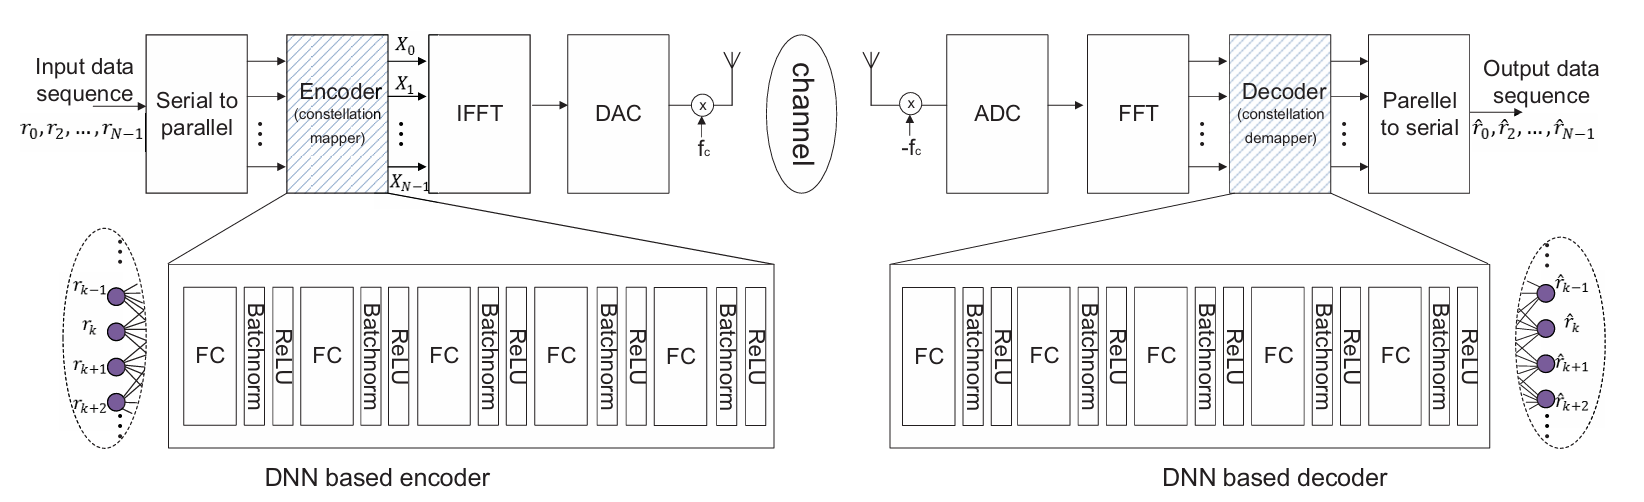
\includegraphics[width=0.95\linewidth]{Figures/PRNet/prnet_architecture.png}
    \caption{Structure of the proposed PRNet with DNN encoder and DNN decoder. Both are stacks of fully connected (FC) layers with Batch Normalization and ReLU activation.  The encoder shapes the constellation before the IFFT to reduce PAPR; the decoder reconstructs the transmitted symbols after the channel and FFT. Reproduced from~\cite{kim2017novel}.}
    \label{fig:prnet_architecture}
\end{figure}

PRNet inserts two trainable Deep Neural Networks (DNNs) around the standard IFFT/FFT pair~\cite{kim2017novel}:
\begin{itemize}
    \item \textbf{Encoder (transmitter-side DNN):} replaces the standard constellation mapper.  Instead of mapping bits to fixed QPSK or QAM points, it takes the input data and produces a new set of complex subcarrier values specifically shaped to yield low peaks after the IFFT.
    \item \textbf{Decoder (receiver-side DNN):} replaces the standard constellation de-mapper.  It takes the received (noisy) frequency-domain subcarriers and directly reconstructs the original data bits.
\end{itemize}

\begin{misconception}
    \textbf{``PRNet replaces the IFFT with a neural network.''} \\
    This is a very common first reaction, but it is incorrect.  The IFFT and FFT are still explicitly present in the signal chain.  They remain fixed, standard mathematical operations sitting inside the PRNet pipeline. What the encoder replaces is the \emph{constellation mapper} --- instead of mapping bits to fixed QPSK points, it maps them to learned complex values that happen to produce lower peaks when passed through the IFFT. The IFFT itself is untouched~\cite{kim2017novel}.
\end{misconception}


\subsection{Why No Side Information Is Needed}

In classical SLM, the receiver must know \emph{which} phase sequence the transmitter selected --- this requires $\lceil\log_2 U\rceil$ bits of side information (SI) per OFDM symbol. If even one of those SI bits arrives in error, the receiver applies the wrong phase reversal and the entire OFDM symbol is destroyed.

PRNet eliminates this vulnerability entirely.  Because the encoder and decoder are trained \emph{jointly} over millions of iterations, the decoder's neural network weights implicitly encode the complete knowledge of what transformation the encoder applies.  The decoder does not need to be told which mapping was used --- it already knows, because it spent the entire training phase learning to invert exactly that mapping~\cite{kim2017novel}.

\begin{keyinsight}[No Side Information Needed]
    In SLM, the decoding rule is external: ``look up which phase sequence was used and reverse it.''  In PRNet, the decoding rule is \emph{internal}: it is baked into the millions of learned weights inside the decoder network. No explicit communication between transmitter and receiver about the mapping is needed.  This completely removes the SI overhead and the catastrophic failure mode of SI errors~\cite{kim2017novel}.
\end{keyinsight}


\subsection{Why the Encoder Sees All Bits Simultaneously}

In standard OFDM with QPSK, the 128 raw bits are chopped into 64 isolated pairs.  Each pair is independently mapped to one of four constellation points, and that point is assigned to a single subcarrier.  Bit pair \#1 knows nothing about bit pair \#2, and subcarrier \#1 knows nothing about what is happening on subcarrier \#2.

PRNet fundamentally breaks this isolation.  The encoder is a \textbf{fully connected (FC)} neural network, which means every single output neuron receives input from every single input neuron.  In the paper's original implementation, the encoder receives the 256-entry one-hot representation of the 64 QPSK symbols, whereas in our continuous I/Q implementation, it receives the 128-entry stacked real/imaginary vector. In both cases, the network sees the whole 128-bit OFDM symbol at once.  Each of the 64 output complex numbers is therefore a function of the \textbf{entire} OFDM input block --- not just the 2 bits that would have been assigned to that subcarrier in standard QPSK~\cite{kim2017novel}.

This holistic processing is what gives PRNet its power.  The encoder can detect dangerous patterns across the full input (e.g., long runs of identical bits that tend to cause constructive interference in the IFFT) and compensate for them by adjusting the amplitudes and phases of \emph{all} 64 subcarriers jointly.

\begin{keyinsight}[Holistic Processing]
    Standard OFDM maps bits to subcarriers independently: 2 bits $\to$ 1 subcarrier.  PRNet maps the full OFDM input block to all subcarriers simultaneously: 64 QPSK symbol categories, or 128 underlying raw bits, $\to$ 64 learned subcarrier values.  This dense dependence is what gives the encoder a chance to avoid PAPR spikes that arise from unfortunate whole-symbol patterns~\cite{kim2017novel}.
\end{keyinsight}


% ============================================================================
\section{System Model: End-to-End Signal Flow}
% ============================================================================

Now let's formalise the complete PRNet signal chain with full mathematical notation.  We will walk through every step from the raw input bits to the recovered output, defining every symbol as it appears.


\subsection{Step 1 --- Preparing the Network Input}

We consider an OFDM system with $N = 64$ subcarriers and QPSK modulation. Each subcarrier transmits a complex constellation point $S_k \in \{+\frac{1}{\sqrt{2}} \pm j \frac{1}{\sqrt{2}}, -\frac{1}{\sqrt{2}} \pm j \frac{1}{\sqrt{2}}\}$, representing $\log_2 4 = 2$ bits. The total number of input bits per OFDM symbol is therefore $N \times 2 = 128$ bits~\cite{kim2017novel}.

In our continuous I/Q coordinate implementation, these $N$ complex symbols are flattened into a real-valued vector $\bm{r} \in \mathbb{R}^{2N}$ by interleaving their real (in-phase, $I$) and imaginary (quadrature, $Q$) components:
\begin{equation*}
    \bm{r} = \left[\mathrm{Re}(S_0),\, \mathrm{Im}(S_0),\, \mathrm{Re}(S_1),\, \mathrm{Im}(S_1),\, \dots,\, \mathrm{Re}(S_{N-1}),\, \mathrm{Im}(S_{N-1})\right]^T \in \mathbb{R}^{128}.
\end{equation*}

For example, if we have $N = 4$ subcarriers and the QPSK symbols are:
\begin{align*}
    S_0 & = +0.707 + j0.707, \\
    S_1 & = -0.707 + j0.707, \\
    S_2 & = -0.707 - j0.707, \\
    S_3 & = +0.707 - j0.707,
\end{align*}
the stacked real-valued input vector $\bm{r}$ is:
\begin{equation*}
    \bm{r} = [\underbrace{0.707,\, 0.707}_{\text{Subcarrier 0}},\;
    \underbrace{-0.707,\, 0.707}_{\text{Subcarrier 1}},\;
    \underbrace{-0.707,\, -0.707}_{\text{Subcarrier 2}},\;
    \underbrace{0.707,\, -0.707}_{\text{Subcarrier 3}}]^T \in \mathbb{R}^8.
\end{equation*}

By representing QPSK symbols directly as continuous real values, the neural network operates directly in the physical signal space. This differs from the paper's original formulation, which maps categorical symbol indices using one-hot encoding, as explained in Section~\ref{sec:representation_comparison}.

\begin{keyinsight}[Why Continuous I/Q Coordinates?]
    Using physical I/Q coordinates allows the neural network's input and output layers to map directly onto the actual complex constellation plane. This maintains mathematical consistency with the physical transceiver components (which transmit I/Q voltages) and avoids adding artificial category classifications or large, sparse boundary matrices to the network.
\end{keyinsight}

\subsection{Step 2 --- The Encoder: Learned Constellation Shaping}

The encoder is a deep neural network that takes the input vector $\bm{r} \in \mathbb{R}^{2N}$ and outputs a vector of $2N = 128$ real numbers.  These 128 numbers represent the real and imaginary parts of 64 complex subcarrier values~\cite{kim2017novel}:

\begin{equation*}
    f(\bm{r};\,\theta_f) \in \mathbb{R}^{2N},
\end{equation*}
where $\theta_f = \{\bm{W}_1^f, \bm{b}_1^f, \dots, \bm{W}_{L_f}^f, \bm{b}_{L_f}^f\}$ denotes all the learnable weights and biases of the encoder.

To use these $2N$ real numbers in the OFDM chain, we must convert them back into $N$ complex symbols.  We define the \textbf{unstacking operator} $\mathcal{C}(\cdot) : \mathbb{R}^{2N} \to \mathbb{C}^{N}$, which pairs up consecutive elements as real and imaginary parts:

\begin{equation*}
    \bm{X}_{\mathrm{enc}} = \mathcal{C}\bigl(f(\bm{r};\,\theta_f)\bigr)
    \in \mathbb{C}^{N},
\end{equation*}
where, concretely, the $k$-th encoded complex symbol is:
\begin{equation*}
    X_{\mathrm{enc},k}
        = [f(\bm{r})]_{2k} + j \cdot [f(\bm{r})]_{2k+1},
    \qquad k = 0, 1, \dots, N-1.
\end{equation*}

These encoded symbols $\bm{X}_{\mathrm{enc}}$ are \emph{not} standard QPSK points.  They are data-dependent, continuous-valued complex numbers that the encoder specifically crafted to produce a low-PAPR waveform after the IFFT. If you were to plot them on a constellation diagram, they would not form the neat four-point QPSK grid --- instead, they would scatter in a seemingly irregular pattern that has been geometrically optimised for the IFFT's physics~\cite{kim2017novel}.

\begin{figure}[H]
    \centering
    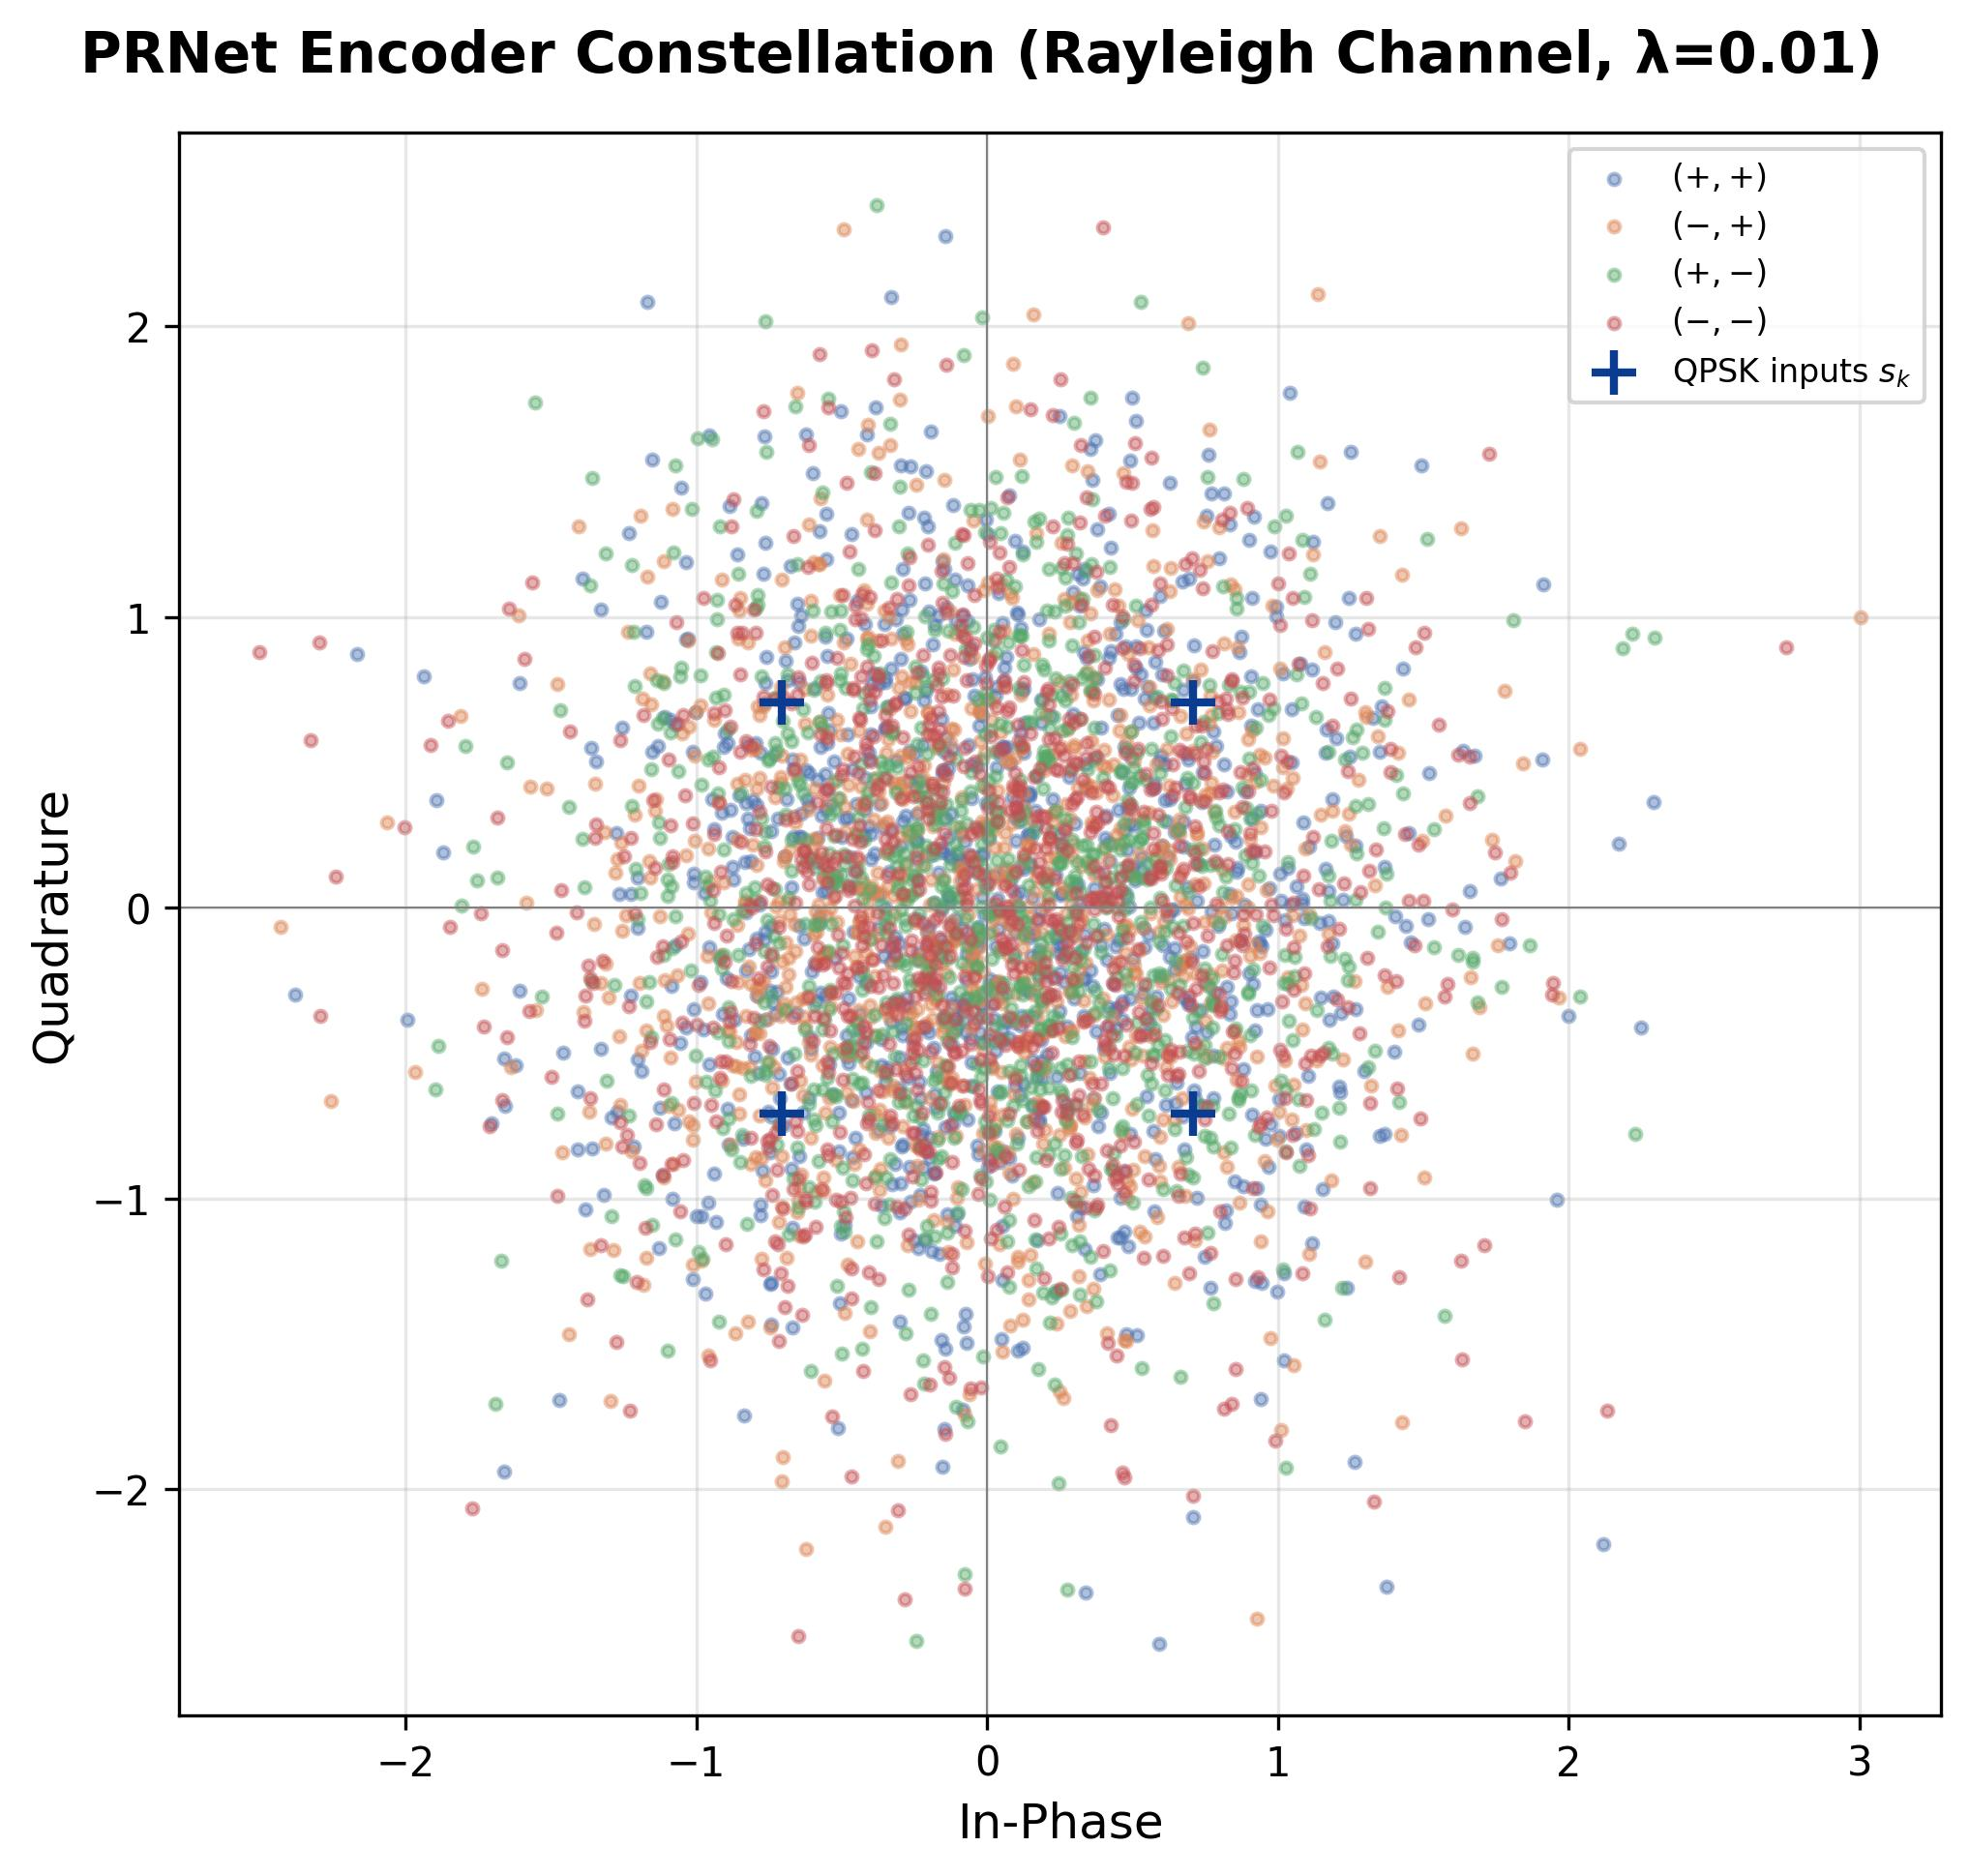
\includegraphics[width=0.6\linewidth]{Figures/PRNet/PRNet - Results/encoder_constellation_rayleigh.jpg}
    \caption{Scatter plot of the encoder's learned constellation. Unlike standard QPSK where symbols are constrained to four fixed points, the PRNet encoder disperses the complex symbols across the constellation plane to minimise PAPR jointly with reconstruction error.}
    \label{fig:prnet_constellation_explanation}
\end{figure}

\begin{workingexample}[What the Encoder's Output Looks Like]
    In standard QPSK, every subcarrier gets one of exactly four points: $\{(+0.707,\,+0.707),\; (+0.707,\,-0.707),\; (-0.707,\,+0.707),\; (-0.707,\,-0.707)\}$. In PRNet, the encoder might output something like $(0.42,\, -0.91)$ for subcarrier \#1, $(-1.13,\, 0.07)$ for subcarrier \#2, $(0.68,\, 0.55)$ for subcarrier \#3, and so on. These are not from any standard constellation --- they are custom values that the network learned will avoid destructive IFFT interactions for this specific input bit pattern.
\end{workingexample}

\subsection{Step 3 --- OFDM Modulation: The Standard IFFT}

The encoded symbols are modulated onto the subcarriers via the standard IFFT~\cite{kim2017novel}:
\begin{keyresult}
    \begin{equation}
        x[n] = \sum_{k=0}^{N-1} X_{\mathrm{enc},k}\, e^{\,j2\pi nk/N},
        \qquad 0 \le n \le N-1.
    \end{equation}
\end{keyresult}

This is the standard IFFT operation --- nothing has changed about OFDM modulation itself.  The only difference is that the complex numbers $X_{\mathrm{enc},k}$ entering the IFFT are no longer fixed QPSK points; they are the encoder's custom-shaped values.

\paragraph{Oversampling.}
PAPR depends on the \emph{maximum} of the continuous-time waveform. If we only compute the IFFT at $N$ samples, we can miss peaks that occur \emph{between} samples.  For a stricter approximation of continuous-time PAPR, the usual approach is to zero-pad the frequency-domain vector from length $N$ to length $NL$, then compute an $NL$-point IFFT.  With $N = 64$ and $L = 4$, this produces $64 \times 4 = 256$ time-domain samples.

This detail needs careful wording for PRNet.  The standard PAPR evaluation in our Rayleigh reproduction uses $L = 4$, because this is the scientifically safer way to estimate peaks.  However, the original paper does not clearly document oversampling in the PRNet CCDF calculation, and the authors' released code effectively evaluates the PRNet waveform on the $N$ IFFT samples.  Oversampling is therefore recommended for standard PAPR reporting, but it is not the reason the paper's red PRNet CCDF curve appears near 3~dB; that discrepancy is explained in the simulation results section below.


\subsection{Step 4 --- The Wireless Channel}

After OFDM modulation, the time-domain signal is transmitted over the wireless channel. The paper models this generally as~\cite{kim2017novel}:
\begin{equation*}
    \bm{y} = \mathbb{H}(\bm{x}) + \bm{\epsilon},
\end{equation*}
where $\mathbb{H}$ denotes the channel effects (Rayleigh fading~\cite{kim2017novel}) and $\bm{\epsilon}$ is additive white Gaussian noise (AWGN) with noise power determined by the signal-to-noise ratio (SNR).

In our coordinate-based Rayleigh implementation, the flat fading channel and noise are modeled directly in the frequency domain per subcarrier as:
\begin{equation*}
    Y_k = H_k X_{\mathrm{enc},k} + E_k,
\end{equation*}
where $H_k \sim \mathcal{CN}(0, 1)$ represents the complex fading channel coefficient for the $k$-th subcarrier, and $E_k$ represents AWGN noise. The receiver then performs Zero-Forcing (ZF) equalization:
\begin{equation*}
    \hat{Y}_k = \frac{Y_k}{H_k} = X_{\mathrm{enc},k} + \frac{E_k}{H_k}.
\end{equation*}
This frequency-domain flat fading with perfect CSI is mathematically equivalent to time-domain flat fading with standard equalization, but simplifies backpropagation through the channel during training.

\begin{keyinsight}[The Channel as a Fixed Mathematical Layer]
    From the neural network's perspective, the channel is not a trainable component --- it is a \emph{fixed mathematical function} sitting in the middle of the computation graph.  During training, the channel is simulated by generating random noise and (optionally) random fading coefficients, and adding them to the transmitted signal.  This simulation allows the gradients from the loss function to flow backward through the channel during backpropagation, because the channel is simply a sequence of differentiable mathematical operations (addition, division, multiplication) applied to the signal~\cite{kim2017novel}.
\end{keyinsight}


\subsection{Step 5 --- OFDM Demodulation and Decoding}

At the receiver, the received time-domain signal $\bm{y}$ passes through the standard FFT to recover the frequency-domain subcarriers:
\begin{equation*}
    \bm{Y} = \mathrm{FFT}(\bm{y}) \in \mathbb{C}^{N}.
\end{equation*}

These received subcarriers are noisy, distorted versions of the encoder's output $\bm{X}_{\mathrm{enc}}$.  Instead of a standard QAM de-mapper (which would look for the nearest QPSK point and reverse the mapping), PRNet feeds them into the \textbf{decoder DNN}.

The decoder first converts the complex equalizer output symbols $\hat{\bm{Y}}$ into a real vector by stacking real and imaginary parts (the inverse of the unstacking we did in Step~2), then processes this real vector through its own deep network to produce the output~\cite{kim2017novel}:
\begin{equation*}
    \hat{\bm{r}} = g\bigl(\mathcal{S}(\hat{\bm{Y}});\,\theta_g\bigr)
    \in \mathbb{R}^{2N},
\end{equation*}
where $\theta_g$ denotes the decoder's learnable parameters and $\mathcal{S}(\cdot) : \mathbb{C}^{N} \to \mathbb{R}^{2N}$ is the \textbf{stacking operator} that interleaves the real and imaginary parts into a single real vector.

The decoder's output $\hat{\bm{r}}$ is a real-valued vector of size $2N = 128$, containing the reconstructed real and imaginary parts of the transmitted QPSK symbols. The final decision is made by passing the reconstructed I/Q coordinates to a nearest-neighbor hard-decision QPSK demodulator:
\begin{equation*}
    \hat{S}_k = \mathrm{sign}(\hat{r}_{2k}) \cdot \frac{1}{\sqrt{2}} + j \cdot \mathrm{sign}(\hat{r}_{2k+1}) \cdot \frac{1}{\sqrt{2}}.
\end{equation*}

\begin{workingexample}[How the Decoder Recovers the Data]
    For subcarrier \#7, the decoder's output might be the coordinate pair $(\hat{r}_{14},\, \hat{r}_{15}) = (-0.68,\, 0.72)$.  The nearest QPSK constellation point is $(-0.707,\, +0.707)$, which corresponds to the bit pair ``10''. The receiver therefore decodes ``10'' for subcarrier \#7. The decoder makes this decision purely from the 64 noisy complex numbers it received --- it was never told what mapping the encoder used.
\end{workingexample}


\subsection{The Complete Chain in One Equation}

The paper expresses the entire end-to-end PRNet chain in one compact equation~\cite{kim2017novel}:
\begin{keyresult}
    \begin{equation}
        \hat{\bm{r}}
        = g \circ \mathrm{FFT} \circ \mathbb{H} \circ \mathrm{IFFT}
        \circ f(\bm{r})
    \end{equation}
\end{keyresult}

Reading this from right to left: the input $\bm{r}$ enters the encoder $f$, passes through the IFFT, travels through the channel $\mathbb{H}$, is demodulated by the FFT, and finally enters the decoder $g$ to produce the reconstructed output $\hat{\bm{r}}$.

The goal of training is to make $\hat{\bm{r}}$ as close to $\bm{r}$ as possible (low BER), while simultaneously ensuring that the IFFT output $x[n]$ has low PAPR.

In short, PRNet wraps the standard OFDM modulation/demodulation chain with two DNNs.  The encoder reshapes the constellation \emph{before} the IFFT to suppress peaks, and the decoder learns to invert that reshaping \emph{after} the channel and FFT.  The IFFT, FFT, and channel are all fixed --- they are not replaced and their equations are unchanged from standard OFDM.

\begin{table}[H]
    \centering
    \caption{Summary of PRNet signal dimensions for the continuous I/Q formulation. With oversampling, $x[n]$ and $\bm{y}$ have length $NL$; with $L=4$ this is 256 samples.}
    \label{tab:prnet_shapes}
    \begin{tabular}{@{} l l l @{}}
        \toprule
        \textbf{Symbol}         & \textbf{Domain / Shape}                     & \textbf{Meaning} \\
        \midrule
        $\bm{r}$                & $\mathbb{R}^{2N}$ ($128$)
                                & Flat real-valued input QPSK symbols                            \\
        $f(\bm{r})$             & $\mathbb{R}^{2N}$ ($128$)
                                & Encoder output (stacked I/Q)                                   \\
        $\bm{X}_{\mathrm{enc}}$ & $\mathbb{C}^{N}$ ($64$)
                                & Encoded complex subcarrier symbols                             \\
        $x[n]$                  & $\mathbb{C}^{NL}$ ($64L$)
                                & IFFT output (time-domain waveform)                             \\
        $\bm{y}$                & $\mathbb{C}^{NL}$ ($64L$)
                                & Received signal (after channel)                                \\
        $\bm{Y}$                & $\mathbb{C}^{N}$ ($64$)
                                & FFT output / Equalizer input                                   \\
        $\hat{\bm{r}}$          & $\mathbb{R}^{2N}$ ($128$)
                                & Decoder output (reconstructed QPSK symbols)                    \\
        \bottomrule
    \end{tabular}
\end{table}


% ============================================================================
\section{Comparative Analysis of Input Representations: One-Hot vs. Continuous I/Q}
\label{sec:representation_comparison}
% ============================================================================

To fully understand the difference between the original paper's setup and our implementation, we need to compare their input representation schemes.

The original PRNet architecture proposed by Kim et al.~\cite{kim2017novel} represents the input data block using a concatenated set of one-hot encoded vectors. For QPSK modulation (constellation size $M=4$) and $N=64$ subcarriers, each subcarrier's data symbol index $r_k \in \{0, 1, 2, 3\}$ is mapped to a $4$-dimensional one-hot vector:
\begin{equation*}
    \text{one-hot}(r_k) = [0,\, \dots,\, 1,\, \dots,\, 0]^T \in \mathbb{R}^4.
\end{equation*}
These individual vectors are concatenated to yield a sparse network input vector $\bm{r}_{\mathrm{one\_hot}} \in \mathbb{R}^{256}$. Symmetrically, the decoder outputs a reconstruction score vector of size $256$, which is optimized using a Mean Squared Error (MSE) loss function.

Conversely, the transceiver implementation investigated in this work utilizes a direct, continuous real-valued vector representation of standard QPSK I/Q coordinates, mapping the $N=64$ complex QPSK symbols directly into an interleaved real vector $\bm{r} \in \mathbb{R}^{128}$ of in-phase ($I$) and quadrature ($Q$) components:
\begin{equation*}
    \bm{r} = \left[\mathrm{Re}(S_0),\, \mathrm{Im}(S_0),\, \dots,\, \mathrm{Re}(S_{N-1}),\, \mathrm{Im}(S_{N-1})\right]^T \in \mathbb{R}^{128}.
\end{equation*}

\subsection{Physical Signalling: Understanding the I/Q Values}
In this continuous formulation, the input values to the neural network are the physical in-phase ($I$) and quadrature ($Q$) components of the QPSK constellation. For standard QPSK, each symbol is normalized to unit average power ($\mathbb{E}[|S|^2] = 1.0$). Therefore, the constellation points are placed at:
\begin{equation*}
    S \in \left\{ +\frac{1}{\sqrt{2}} \pm j \frac{1}{\sqrt{2}},\, -\frac{1}{\sqrt{2}} \pm j \frac{1}{\sqrt{2}} \right\} \approx \{ +0.707 \pm j 0.707,\, -0.707 \pm j 0.707 \}.
\end{equation*}
This means the input vector $\bm{r}$ consists exclusively of values that are either $+0.707$ or $-0.707$. 

\begin{misconception}
    \textbf{``Inputs to a neural network must always be between 0 and 1.''} \\
    It is a common training tip that inputs should be normalized, which leads many to believe they must lie strictly between $0$ and $1$ (the reason behind one-hot encoding). 
    
    However, neural networks mathematically perform much better when inputs are \textbf{zero-centered} (having a mean of $0.0$) and scaled to a standard variance (ranging roughly between $-1.0$ and $+1.0$). Our continuous $I/Q$ values of $+0.707$ and $-0.707$ satisfy this perfectly: they have a mean of $0.0$, a standard deviation of $0.707$, and are perfectly zero-centered, making them ideal for backpropagation without requiring any one-hot formatting.
\end{misconception}

\subsection{Vector Assembly: How the Network Tells Real and Imaginary Apart}
Because standard deep learning libraries only process real numbers, we pass the real and imaginary parts of the complex symbols together in a single real vector. In our implementation, they are interleaved:
\begin{itemize}
    \item \textbf{Even indices} ($0, 2, 4, \dots, 2N-2$) represent the In-Phase (Real) parts.
    \item \textbf{Odd indices} ($1, 3, 5, \dots, 2N-1$) represent the Quadrature (Imaginary) parts.
\end{itemize}

The network does not possess an innate logical understanding of complex numbers, nor do we write explicit code telling it how the indices are related. Instead, the network relies on the \textbf{deterministic spatial arrangement} of the inputs. Because the real part of subcarrier $k$ is always at index $2k$, and the imaginary part is always at index $2k+1$, the weights connected to these indices learn to process them consistently during training.

\subsection{Solving Coordinate Conflicts: How Multiple Neurons Distinguish Symbols}
If we look at a single subcarrier's $I/Q$ coordinate pair, a single hidden neuron with weights $W_I$ and $W_Q$ cannot distinguish all four QPSK states on its own. For example, if a neuron has weights $W_I = 1.0$ and $W_Q = -1.0$, the combined output for opposite symbols becomes identical:
\begin{itemize}
    \item \textbf{Symbol 0} ($+0.707, +0.707$) $\to 1.0(0.707) - 1.0(0.707) = 0.0$
    \item \textbf{Symbol 3} ($-0.707, -0.707$) $\to 1.0(-0.707) - 1.0(-0.707) = 0.0$
\end{itemize}

However, PRNet resolves this by using multiple neurons in each layer ($K = 2048$ nodes). By projecting the coordinates through multiple different sets of weights, the network views the inputs from different angles. Consider two hidden neurons:
\begin{itemize}
    \item \textbf{Neuron 1} weights: $W_I^{(1)} = 1.0$, $W_Q^{(1)} = -1.0$
    \item \textbf{Neuron 2} weights: $W_I^{(2)} = 1.0$, $W_Q^{(2)} = 1.0$
\end{itemize}

The activations of these two neurons form an output vector $\bm{h} = [h_1, h_2]^T$ that uniquely identifies each QPSK symbol:
\begin{table}[H]
    \centering
    \caption{Multi-neuron activation mapping for QPSK symbols.}
    \begin{tabular}{lcccc}
        \toprule
        Symbol & Coordinates $(I, Q)$ & Neuron 1 Output & Neuron 2 Output & Combined Activation Vector \\
        \midrule
        Symbol 0 & $(+0.707, +0.707)$ & $0.0$ & $+1.414$ & $\begin{bmatrix} 0.0 & +1.414 \end{bmatrix}^T$ \\
        Symbol 1 & $(+0.707, -0.707)$ & $+1.414$ & $0.0$ & $\begin{bmatrix} +1.414 & 0.0 \end{bmatrix}^T$ \\
        Symbol 2 & $(-0.707, +0.707)$ & $-1.414$ & $0.0$ & $\begin{bmatrix} -1.414 & 0.0 \end{bmatrix}^T$ \\
        Symbol 3 & $(-0.707, -0.707)$ & $0.0$ & $-1.414$ & $\begin{bmatrix} 0.0 & -1.414 \end{bmatrix}^T$ \\
        \bottomrule
    \end{tabular}
    \label{tab:multi_neuron_mapping}
\end{table}
Subsequent layers of the network look at these combined activation coordinates and can easily decode or shape the symbol boundaries without any ambiguity.

\begin{keyinsight}[Why One-Hot and Continuous Representations Are Equivalent]
    Because a standard QPSK constellation consists of four orthogonal coordinates in the 2D plane:
    \begin{equation*}
        S \in \left\{ +\frac{1}{\sqrt{2}} \pm j \frac{1}{\sqrt{2}},\, -\frac{1}{\sqrt{2}} \pm j \frac{1}{\sqrt{2}} \right\},
    \end{equation*}
    the mapping between the $4$-dimensional one-hot vector and the 2D physical coordinates is strictly linear. For instance, if the one-hot categories represent the indices $\{0,1,2,3\}$, a simple matrix multiplication can map them directly to the coordinate plane:
    \begin{equation*}
        \begin{bmatrix} I \\ Q \end{bmatrix} = \frac{1}{\sqrt{2}}\begin{bmatrix} 1 & -1 & -1 & 1 \\ 1 & 1 & -1 & -1 \end{bmatrix} \begin{bmatrix} x_0 \\ x_1 \\ x_2 \\ x_3 \end{bmatrix},
    \end{equation*}
    where $[x_0, x_1, x_2, x_3]^T$ is the one-hot vector. Because the first layer of the neural network has a wide hidden dimension of $K=2048$ nodes, it can trivially learn this linear mapping inside its input weight matrix. The same logic holds for the decoder's output layer. Thus, both formulations are informationally equivalent and yield identical BER and CCDF performance.
\end{keyinsight}

Despite their equivalence in results, the continuous I/Q representation offers three critical engineering advantages:
\begin{itemize}
    \item \textbf{Dimensionality Reduction:} The input layer is reduced from $256$ to $128$ dimensions, which cuts the parameter size of the first projection matrix in half (from $256 \times 2048$ to $128 \times 2048$ weights).
    \item \textbf{Transceiver Simplification:} Bypassing one-hot encoding eliminates the need for categorical mapping and de-mapping layers at the boundaries of the neural network, allowing the model to operate directly in the physical signal domain.
    \item \textbf{Strict Power Normalization:} The continuous I/Q representation allows power normalization to be applied per individual OFDM symbol in the batch, ensuring that the average power constraint $\mathbb{E}[|X|^2] = 1.0$ is strictly enforced for every transmitted waveform. In contrast, the paper's original one-hot code enforces normalization globally across the entire training batch, allowing individual OFDM symbols to experience power fluctuations.
\end{itemize}

\subsection{Weight Dynamics: Evolving During Training}
The weights in these neurons are the parameters that define the network's behavior. They are not fixed numbers; they change dynamically throughout the training process:
\begin{itemize}
    \item \textbf{Initialization:} To prevent activation explosion, weights are initialized to small random numbers. Using Xavier or He initialization, the weights for a hidden layer with 2048 nodes are initialized in a narrow range around $\pm 0.038$.
    \item \textbf{Training Updates:} Throughout training, gradients are calculated via backpropagation, and the optimizer updates the weights to minimize the loss (joint BER and PAPR reduction):
      \begin{equation*}
          W_{\mathrm{new}} := W_{\mathrm{old}} - \alpha \nabla_{W} \mathcal{L}.
      \end{equation*}
    \item \textbf{Final Range:} After training, the weights converge to stable distributions. While the majority of weights remain small (concentrated between $-0.5$ and $+0.5$), some crucial weights grow to larger values (e.g., reaching $-2.0$ or $+2.0$). To keep these weights from growing uncontrollably (which could lead to overfitting or high noise sensitivity), we apply \textbf{L2 Regularization} (weight decay), which penalizes large weights and keeps the network stable.
\end{itemize}


% ============================================================================
\section{Network Architecture: FC + BatchNorm + ReLU}
% ============================================================================

Now that we understand what the encoder and decoder are supposed to do, let's look at how they are built internally. Both networks have \emph{identical} architectures composed of repeated sub-blocks, each consisting of three operations applied in sequence~\cite{kim2017novel}.

\subsection{The Sub-Block: One Layer of Processing}

Each sub-block transforms an input vector $\bm{h}^{(\ell-1)}$ into an output vector $\bm{h}^{(\ell)}$ through three stages:

\paragraph{Stage 1 --- Fully Connected (FC) Layer.}
A fully connected layer (also called a dense layer) is a simple linear transformation where every input neuron is connected to every output neuron: it multiplies the input by a weight matrix and adds a bias vector. For a layer with $d_{\mathrm{in}}$ inputs and $d_{\mathrm{out}}$ outputs, the computation is~\cite{kim2017novel}:

\begin{equation*}
    \bm{y}_{\mathrm{FC}} = \bm{W}_m \bm{h}^{(\ell-1)} + \bm{b}_m,
\end{equation*}
where $\bm{W}_m \in \mathbb{R}^{d_{\mathrm{out}} \times d_{\mathrm{in}}}$ is the weight matrix and $\bm{b}_m \in \mathbb{R}^{d_{\mathrm{out}}}$ is the bias vector for the $m$-th sub-block. The hidden FC layers in PRNet use $2048$ nodes --- meaning $d_{\mathrm{out}} = 2048$ for those layers, so a hidden weight matrix has $2048 \times d_{\mathrm{in}}$ entries. These are the primary learnable parameters of the network~\cite{kim2017novel}.

\paragraph{Stage 2 --- Batch Normalization (BN).}
As data flows through many layers in a deep neural network, the distribution of each layer's input can shift dramatically during training (a phenomenon called \textbf{internal covariate shift}). Batch Normalization fixes this by normalising the FC output to have zero mean and unit variance within each training mini-batch, then applying a learnable scale and shift~\cite{kim2017novel}:

\begin{equation*}
    |\bm{y}_{\mathrm{FC}}|_{\mathrm{norm}}
    = \gamma \cdot
    \frac{\bm{y}_{\mathrm{FC}} - \mathbb{E}[\bm{y}_{\mathrm{FC}}]}
    {\sqrt{\mathrm{Var}[\bm{y}_{\mathrm{FC}}] + \nu}}
    + \beta,
\end{equation*}
where $\gamma$ is a learnable scaling parameter, $\beta$ is a learnable shifting parameter, and $\nu = 0.001$ is a small constant to prevent division by zero~\cite{kim2017novel}.

The practical effect is significant: without BatchNorm, training a 5-layer deep network is extremely slow because each layer's output statistics keep changing, forcing subsequent layers to constantly readapt. BatchNorm stabilises these statistics, allowing the use of higher learning rates and dramatically speeding up convergence.

\paragraph{Stage 3 --- ReLU Activation.}
After normalisation, the values pass through the \textbf{Rectified Linear Unit} (ReLU) activation function~\cite{kim2017novel}:
\begin{equation*}
    \phi(x) = \max(x,\, 0).
\end{equation*}

ReLU provides the \emph{nonlinearity} that is absolutely essential for PRNet to work.

\begin{keyinsight}[Why Nonlinearity Is Essential]
    Without nonlinear activation functions, no matter how many FC layers we stack, the entire network would collapse into a single matrix multiplication: $\bm{W}_5 \bm{W}_4 \bm{W}_3 \bm{W}_2 \bm{W}_1 \bm{r} + \bm{b} = \bm{W}_{\mathrm{equiv}} \bm{r} + \bm{b}$. A single linear transformation can only rotate and scale the constellation --- it cannot perform the complex, nonlinear warping required to simultaneously avoid all PAPR-inducing patterns.  The paper explicitly notes that the constellation shaping problem is a ``multivariate non-convex problem that is NP-hard''~\cite{kim2017novel}, which means no linear method can solve it.  ReLU is what gives the network the expressive power to learn the nonlinear mapping.
\end{keyinsight}


\subsection{The Complete Sub-Block}

Putting all three stages together, the transformation performed by the $\ell$-th sub-block is~\cite{kim2017novel}:
\begin{equation*}
    \bm{h}^{(\ell)}
    = \phi\!\Bigl(
    \mathrm{BN}\bigl(\bm{W}^{(\ell)}\bm{h}^{(\ell-1)}
        + \bm{b}^{(\ell)}\bigr)
    \Bigr),
    \qquad \phi(\cdot) = \mathrm{ReLU}(\cdot).
\end{equation*}


\subsection{Full Encoder and Decoder}

The paper describes the encoder as $L_f = 5$ FC--BN--ReLU sub-blocks chained together.  Its mathematical expression is~\cite{kim2017novel}:
\begin{keyresult}
    \begin{equation}
        f(\bm{r})
        = \phi_{L_f}\!\Bigl(
        \bigl|\bm{W}_{L_f}^f\,
        \phi_{L_f-1}\bigl(\cdots
        \phi_1\bigl(|\bm{W}_1^f\,\bm{r}
            + \bm{b}_1^f|_{\mathrm{norm}}\bigr)
        \cdots\bigr)
        + \bm{b}_{L_f}^f\bigr|_{\mathrm{norm}}
        \Bigr),
    \end{equation}
\end{keyresult}
where $\bm{W}_{l_f}^f$ and $\bm{b}_{l_f}^f$ are the weights and biases of the $l_f$-th FC in the encoder, and $|\cdot|_{\mathrm{norm}}$ denotes the batch normalisation operation.

The decoder has the exact same structure --- $L_g = 5$ sub-blocks --- but with its own separate set of weights and biases ($\bm{W}_{l_g}^g$, $\bm{b}_{l_g}^g$).  The encoder and decoder are symmetric in topology but \textbf{not} in learned weights --- each network independently discovers its own optimal parameters during training~\cite{kim2017novel}.

\paragraph{Critique of the Final Output Layer.}
Crucially, while the paper's literal formula in Equation (2.3) (and shown in our Eq.~(2.3) above) includes the activation function $\phi_{L_f}$ (ReLU) and Batch Normalization at the final output layer, the practical implementation in the authors' released code (and our reproduction) deviates from this. The final output layer of both the encoder and decoder is a pure fully connected layer with a \textbf{linear activation function} and \textbf{no Batch Normalization}.

Why is this deviation necessary?
\begin{itemize}
    \item \textbf{Avoiding ReLU Clamping:} The output values of both networks must be allowed to span any positive or negative real value. The encoder needs to produce arbitrary positive and negative I/Q coordinates, and the decoder needs to produce arbitrary coordinates (or scores). If we applied a ReLU activation ($\max(x, 0)$) at the final layer, all negative outputs would be clamped to zero, completely destroying half of the signal space.
    \item \textbf{Omitting Batch Normalization:} Batch Normalization forces the outputs to have a zero mean and unit variance across a batch. If applied at the very end of the encoder, it would interfere with the average power normalization, and if applied at the end of the decoder, it would warp the reconstructed constellation amplitudes.
\end{itemize}

In short, each encoder and decoder is a deep FC network with 2048-node hidden processing blocks, BatchNorm, ReLU nonlinearities, and a linear output projection for the final transmitted I/Q values or reconstructed symbol coordinates. The nonlinear hidden stack gives the network enough expressive power to learn the complex, NP-hard constellation shaping that reduces PAPR.


% ============================================================================
\section{The Loss Function and Training Procedure}
% ============================================================================

Now we arrive at the core of PRNet: \emph{how} the encoder and decoder actually learn.  The key challenge is that we must optimise for two competing objectives simultaneously --- and the tension between them is what makes PRNet's training procedure so carefully designed.

\subsection{Two Competing Objectives}

Let's state the two goals plainly before introducing any math:

\begin{enumerate}
    \item \textbf{Objective 1 --- Recoverability (low BER):} The decoder must reliably reconstruct the original data from the noisy received signal.  If we only cared about this, we would train a standard autoencoder --- it would learn to survive channel noise, but would do nothing about PAPR.
    \item \textbf{Objective 2 --- Peak suppression (low PAPR):} The encoder's output must produce a time-domain waveform with low peaks after the IFFT.  If we only cared about this, we could flatten the signal entirely to a constant envelope --- but then all subcarriers would carry the same information, and the decoder would have no way to distinguish different bit patterns.
\end{enumerate}

These two objectives are fundamentally in tension: aggressively reducing PAPR requires distorting the constellation geometry, which makes the decoder's job harder and increases BER.  PRNet manages this tension through a carefully designed \textbf{joint loss function} that balances both goals~\cite{kim2017novel}.

\subsection{Loss~1 --- Reconstruction Loss (MSE)}

The first loss function measures how well the decoder recovers the original input.  It computes the \textbf{Mean Squared Error (MSE)} between the original input vector $\bm{r}$ and the decoder's output $\hat{\bm{r}}$ in the $2N$-dimensional real space~\cite{kim2017novel}:

\begin{keyresult}
    \begin{equation}
        \mathcal{L}_1(\bm{r},\hat{\bm{r}})
        = \frac{1}{2N}\|\bm{r} - \hat{\bm{r}}\|_2^2
        = \frac{1}{2N}\sum_{i=0}^{2N-1}\bigl(r_i - \hat{r}_i\bigr)^2.
    \end{equation}
\end{keyresult}

This is the standard autoencoder reconstruction loss.  It computes the squared difference between each element of the original QPSK input vector and the decoder's corresponding output, then averages over all $2N$ (128) elements.

When this loss is large, it means the decoder is producing outputs that are far from the original data --- in other words, many bits are being decoded incorrectly.  When this loss is small, the decoder is accurately recovering the transmitted data, which translates directly to low BER.

\begin{keyinsight}[Why MSE and Not Cross-Entropy?]
    In classification problems (e.g., ``is this image a cat or a dog?''), cross-entropy is the standard loss function. Because the paper trains PRNet as an autoencoder that reconstructs its input vector directly, it uses MSE between the target input vector and the decoder's output. In our continuous I/Q implementation, this is MSE in the 128-dimensional coordinate space, representing the physical distance between transmitted and received constellation points.
\end{keyinsight}

\subsection{Loss~2 --- PAPR Penalty}

The second loss function directly measures the PAPR of the time-domain waveform.  PAPR is the ratio of peak instantaneous power to average power. Written with an explicit oversampling factor $L$, the standard power-PAPR loss is:

\begin{keyresult}
    \begin{equation}
        \mathcal{L}_2(\bm{r})
        = \mathrm{PAPR}\{x[n]\}
        = \frac{\displaystyle\max_{0 \le n \le NL-1} |x[n]|^2}
        {\displaystyle\frac{1}{NL}\sum_{n=0}^{NL-1}|x[n]|^2}.
    \end{equation}
\end{keyresult}

For scientifically strict reporting, both the maximum and the mean should be computed over the oversampled waveform.  In the original paper, Eq.~(6) writes the PAPR term compactly as $\mathrm{PAPR}\{\mathrm{IFFT}(f(\bm{r}))\}$ without stating the oversampling detail.  Our Rayleigh reproduction trains the PAPR term with $L=4$ and uses the physical power ratio above.  This loss term is what actively pushes the encoder to shape the constellation such that the IFFT output has smaller peaks.

\begin{keyinsight}[How Gradients Flow Through PAPR]
    At first glance, computing a gradient through the $\max$ function might seem impossible.  But in practice, $\max$ is differentiable almost everywhere --- its gradient is simply 1 at the position of the maximum and 0 everywhere else.  The gradient tells the encoder: ``the peak power occurred at time sample $n^*$; the subcarrier values that contributed most to sample $n^*$ should be adjusted.'' Through the chain rule, this gradient propagates backward through the IFFT (which is just a linear operation) all the way to the encoder's weights~\cite{kim2017novel}.
\end{keyinsight}


\subsection{The Joint Loss Function}

The final PRNet loss is a weighted sum of the two individual losses (paper Eq.~(7))~\cite{kim2017novel}:
\begin{keyresult}
    \begin{equation}
        \mathcal{L}(\bm{r},\hat{\bm{r}})
        = \mathcal{L}_1(\bm{r},\hat{\bm{r}}) + \lambda\,\mathcal{L}_2(\bm{r}),
    \end{equation}
\end{keyresult}
where $\lambda > 0$ is a scalar weight that controls the trade-off between reconstruction accuracy and PAPR reduction.

Let's understand exactly what $\lambda$ does:

\begin{itemize}
    \item \textbf{If $\lambda = 0$:} The PAPR penalty is completely ignored. The network is trained as a pure autoencoder.  It will reconstruct symbols perfectly but will not reduce PAPR at all.
    \item \textbf{If $\lambda$ is very large (e.g., $\lambda = 1$):} The PAPR penalty dominates.  The encoder is pushed extremely hard to flatten the time-domain waveform, but this aggressive constellation distortion makes it nearly impossible for the decoder to distinguish between different bit patterns.  BER skyrockets.
    \item \textbf{If $\lambda = 0.01$ (the paper's chosen value):} The PAPR term is multiplied by $10^{-2}$ before being added to the reconstruction term.  The actual balance depends on the numerical scales of $\mathcal{L}_1$ and $\mathcal{L}_2$, but empirically this value lets the encoder focus primarily on decodability while still nudging the constellation toward lower peaks~\cite{kim2017novel}.
\end{itemize}

\begin{keyinsight}[The $\lambda$ Knob]
    $\lambda$ is the single most important hyperparameter in PRNet. It controls a fundamental, inescapable trade-off: \emph{more PAPR reduction necessarily costs some BER performance, and vice versa.} This trade-off is not a flaw of PRNet --- it is a physical reality of the OFDM system.  Any method that claims to reduce PAPR without any BER cost is either adding redundancy (like coding) or is operating in a regime where the PAPR reduction is minimal~\cite{kim2017novel}.
\end{keyinsight}


\subsection{Two-Stage Training Procedure}

PRNet is trained as a \textbf{denoising autoencoder}: during training, noise is deliberately injected into the signal (simulating the channel) so that the decoder learns a robust inverse mapping that can handle real channel conditions.  The amount of training noise is controlled by the \textbf{corruption level} $\eta$~\cite{kim2017novel}:

\begin{equation*}
    \eta = \frac{\mathbb{E}\bigl[|\epsilon|^2\bigr]}
    {\mathbb{E}\bigl[|\bm{r}|^2\bigr]},
\end{equation*}
where $\epsilon$ is the injected noise power and $\bm{r}$ is the signal power.  This is essentially a noise-to-signal ratio, expressed in dB. For example, $\eta = -15$~dB means the noise power is $10^{-1.5} \approx 0.032$ times the signal power --- a relatively mild corruption.

Choosing $\eta$ correctly is critical, because it determines the size of the ``noise region'' that the decoder must learn to handle around each constellation point~\cite{kim2017novel}:

\begin{itemize}
    \item \textbf{Too little noise ($\eta$ very negative, e.g., $-30$~dB):} The decoder only learns to recover symbols from a tiny noise region very close to each constellation point.  At test time, when real channel noise is larger than what the network trained on, the decoder encounters unfamiliar distortion and fails.
    \item \textbf{Too much noise ($\eta$ too high, e.g., $0$~dB):} The noise regions of adjacent constellation points overlap heavily during training.  The decoder becomes confused and cannot learn to reliably distinguish between neighbouring points.
    \item \textbf{The sweet spot ($\eta = -15$~dB):} The noise is strong enough that the decoder learns robust decision boundaries, but weak enough that the constellation points remain distinguishable during training.
\end{itemize}

To find this sweet spot, Kim et al.\ use a \textbf{two-stage training procedure}~\cite{kim2017novel}:

\begin{enumerate}
    \item \textbf{Stage 1 --- Choose $\eta^\star$ (reconstruction only):} Train multiple separate PRNet models using \emph{only} the reconstruction loss $\mathcal{L}_1$ (i.e., $\lambda = 0$, no PAPR penalty) for a range of $\eta$ values (e.g., $\eta \in \{0, -5, -10, -15, -20, -25, -30\}$~dB). After training each model, evaluate its BER across a full SNR sweep. Select the $\eta$ that yields the lowest overall BER. The paper finds $\eta^\star = -15$~dB~\cite{kim2017novel}.

    \item \textbf{Stage 2 --- Joint training at $\eta^\star$:} Fix $\eta = \eta^\star = -15$~dB and train the final PRNet with the full joint loss $\mathcal{L} = \mathcal{L}_1 + \lambda\,\mathcal{L}_2$. This is the final model that simultaneously reduces PAPR and maintains low BER~\cite{kim2017novel}.
\end{enumerate}

\begin{algorithm}[H]
    \DontPrintSemicolon
    \SetAlgoLined
    \SetKwInOut{Input}{Input}
    \SetKwInOut{Output}{Output}
    \Input{Candidate corruption levels $\{\eta\}$, PAPR weight $\lambda$,
        steps $T$, batch size $B$}
    \Output{Trained parameters $(\theta_f,\theta_g)$}
    \BlankLine
    \tcp{Stage 1: select $\eta^\star$ using $\lambda=0$}
    \ForEach{$\eta$ in $\{\eta\}$}{
        Initialise PRNet parameters $(\theta_f,\theta_g)$\;
        \For{$t=1$ \KwTo $T$}{
            Sample a batch of $B$ random standard QPSK symbols $\to \bm{r}$\;
            Forward pass: $\hat{\bm{r}} \leftarrow
                \mathrm{PRNet}(\bm{r};\theta_f,\theta_g,\eta)$\;
            Compute $\mathcal{L}_1(\bm{r},\hat{\bm{r}})$ and update
            $(\theta_f,\theta_g)$ via Adam\;
        }
        Evaluate BER over an SNR sweep and record result for this $\eta$\;
    }
    Select $\eta^\star$ that minimises BER\;

    \BlankLine
    \tcp{Stage 2: joint training at $\eta^\star$}
    Initialise the final PRNet parameters $(\theta_f,\theta_g)$\;
    \For{$t=1$ \KwTo $T$}{
        Sample a batch of $B$ random standard QPSK symbols $\to \bm{r}$\;
        Forward pass: obtain $\hat{\bm{r}}$ and time-domain $x[n]$\;
        Compute $\mathcal{L} = \mathcal{L}_1(\bm{r},\hat{\bm{r}})
            + \lambda\,\mathcal{L}_2(x[n])$\;
        Update $(\theta_f,\theta_g)$ via Adam on $\nabla\mathcal{L}$\;
    }
    \caption{Two-stage PRNet training procedure~\cite{kim2017novel}.}
    \label{alg:prnet_training}
\end{algorithm}

The reason for separating the two stages is pedagogical and practical. Stage~1 ensures the decoder develops solid noise-handling foundations \emph{before} the encoder starts actively distorting the constellation for PAPR reduction.  If we started with the PAPR penalty active from the very beginning, the encoder would immediately start warping the constellation, but the decoder --- which has random, untrained weights --- would have no ability to follow those distortions.  The result would be chaotic, with neither objective being optimised properly.

In short, Stage~1 builds robust reconstruction capability; Stage~2 then carefully introduces the PAPR objective on top of that solid foundation.


\subsection{Backpropagation Through the Channel}

A natural question arises: ``How can we backpropagate gradients through the wireless channel?  The channel is a physical process, not a neural network layer.''

\begin{misconception}
    \textbf{``You cannot backpropagate through a channel.''} \\
    For an AWGN channel, the received signal is $\bm{y} = \bm{x} + \bm{\epsilon}$, where $\bm{\epsilon}$ is random noise that does \emph{not} depend on the encoder's parameters. The gradient of the loss with respect to $\bm{x}$ is simply $\partial\mathcal{L}/\partial\bm{x} = \partial\mathcal{L}/\partial\bm{y}$, because $\partial(\bm{x} + \bm{\epsilon})/\partial\bm{x} = 1$ --- the additive noise passes through as a constant during differentiation~\cite{kim2017novel}.

    Even for a multiplicative fading channel ($\bm{y} = h\bm{x} + \bm{\epsilon}$), the backpropagated gradient is scaled by the channel coefficient (more precisely, by the adjoint coefficient $h^*$ in complex notation).  This is perfectly computable as long as the fading coefficient $h$ is sampled independently of the transmitted signal and treated as fixed during that forward/backward pass. The channel acts as a known differentiable layer~\cite{kim2017novel}.
\end{misconception}

The same applies to the IFFT and FFT: they are linear operations (matrix multiplications by the DFT matrix), and the gradient of a linear operation is simply its transpose.  So gradients flow cleanly from the loss function backward through the decoder, through the FFT, through the channel, through the IFFT, and all the way back to the encoder's first weight matrix.  Every single weight in the entire system gets a gradient signal telling it how to adjust.


\subsection{Stepping Through the First Training Iterations}

To truly understand \emph{how} PRNet learns, it helps to walk through the very first training iterations in detail.  This reveals how the system goes from complete chaos to a highly optimised mapping.

\subsubsection{Iteration 1: The Chaos Phase}

Before any data is processed, the system initialises.  Every single weight and bias inside both the encoder and decoder is set to a small, completely random number (using Xavier initialisation~\cite{kim2017novel}).  At this point, the network is essentially performing meaningless arithmetic.

\begin{enumerate}
    \item \textbf{Generate input:} We generate a batch of 400 random QPSK symbol sequences. Each sequence consists of 64 random symbols (128 random bits), represented as a 128-dimensional real vector $\bm{r}$ of stacked I/Q coordinates.
    \item \textbf{Encoder (random math):} The 128-element input vector enters the encoder.  Because the weights are random, the five FC~$\to$~BN~$\to$~ReLU layers perform meaningless matrix multiplications.  The encoder outputs 128 real numbers that bear no meaningful relationship to the input bits --- they are essentially random I/Q values.
    \item \textbf{IFFT:} These 64 random complex numbers enter the standard IFFT. Because the numbers are random, some of them will likely align constructively, producing a time-domain waveform with a massive power spike.  The PAPR is very high.
    \item \textbf{Channel:} We simulate the channel by mathematically adding complex Gaussian noise at the level dictated by $\eta = -15$~dB. The signal is now both high-PAPR \emph{and} noisy.
    \item \textbf{FFT:} The noisy time-domain signal is converted back into 64 complex numbers via the FFT.  These are noisy, corrupted versions of the encoder's already-random output.
    \item \textbf{Decoder (random guessing):} The decoder receives these 64 corrupted complex numbers (stacked into a 128-element real vector) and passes them through its own random weights.  Its 128-element output is essentially random: each coordinate pair for each subcarrier is an unstructured set of values, so the nearest-neighbor decision is roughly a uniform random guess among the four QPSK symbols.
    \item \textbf{Loss calculation:} The system evaluates its performance:
          \begin{itemize}
              \item \textbf{Reconstruction loss $\mathcal{L}_1$:} The MSE between the original QPSK I/Q input coordinates and the decoder's random output coordinates is enormous --- the decoder is getting most bits wrong.
              \item \textbf{PAPR loss $\mathcal{L}_2$:} The PAPR of the time-domain waveform is very high (often equivalent to 10+ dB when expressed in dB).
              \item \textbf{Total loss:} $\mathcal{L} = \mathcal{L}_1 + 0.01 \times \mathcal{L}_2$ = a very large number.
          \end{itemize}
    \item \textbf{Backpropagation:} The system takes this total loss and works backward through the entire chain using the chain rule.  For every single weight in both the encoder and decoder, it computes the gradient: ``If I had shifted this specific weight by a tiny amount, would the total loss have been slightly lower or slightly higher?''  It then updates each weight by a small step (controlled by the Adam optimiser's learning rate of $10^{-4}$) in the direction that reduces the loss.
\end{enumerate}

After this first iteration, the 400 input sequences are \textbf{discarded}. They were training examples, not real data.  The only thing that persists is the tiny adjustment made to the weights.

\subsubsection{Iteration 2: The First Micro-Improvement}

A brand new batch of 400 random sequences is generated.  The same process repeats, but now the weights have been nudged slightly:

\begin{itemize}
    \item The encoder's output is infinitesimally less chaotic --- perhaps one or two of the 64 complex numbers are now in slightly more favourable positions.
    \item The PAPR might be 0.01\% lower than it would have been with the original random weights.
    \item The decoder might correctly identify 65 out of 128 bits instead of the expected 64 from pure chance.
    \item The total loss is still massive, but measurably lower than Iteration~1.
\end{itemize}

Backpropagation runs again, computing new gradients based on this specific batch, and nudges the weights another tiny step.

\subsubsection{Iterations 3 through 500{,}000: Building the Mapping}

This exact loop repeats 500{,}000 times.  With each iteration:
\begin{itemize}
    \item \textbf{The encoder's weights migrate} toward mathematical operations that consistently produce complex numbers avoiding constructive interference in the IFFT. Over tens of thousands of gradient updates, each weight settles into a value that contributes to ``safe'' constellation shapes.

    \item \textbf{The decoder's weights migrate} toward operations that can reliably decode the specific, non-standard constellation shapes that the encoder is settling on --- even through channel noise. The encoder and decoder are co-evolving: as the encoder changes its mapping, the decoder adapts, and vice versa.
\end{itemize}

By the end of training, the weights have converged. The total loss is orders of magnitude smaller than at Iteration~1. The encoder now produces a consistent, deterministic mapping from any 128-bit input to 64 complex numbers that yield low PAPR, and the decoder can reliably reconstruct the original bits from the noisy received versions of those complex numbers.

\begin{workingexample}[The Scale of Training]
    With 500{,}000 iterations and a batch size of 400, the network processes $500{,}000 \times 400 = 200{,}000{,}000$ (200 million) random OFDM symbols during training. Each symbol consists of 128 bits, so the network sees $200{,}000{,}000 \times 128 = 25.6 \times 10^9$ total bits. Yet the input space has $2^{128} \approx 3.4 \times 10^{38}$ possible bit sequences --- the network sees only a vanishingly small fraction. Despite this, it learns to handle \textbf{all} possible inputs through generalisation: it discovers the underlying geometric rules of PAPR avoidance, not a memorised lookup table.
\end{workingexample}

In short, training is a process of gradual, iterative refinement. The system starts from complete randomness and, through millions of tiny gradient-guided corrections, sculpts its weights into a precise mathematical function that maps any input bit sequence to a low-PAPR constellation shape while remaining decodable through channel noise.


% ============================================================================
\section{The Deployed System: Inference, Generalization, and Resilience}
% ============================================================================

Once training is complete, the system transitions from the laboratory phase to the deployment phase. This transition changes the system's behaviour fundamentally.


\subsection{Frozen Weights and Pure Forward Passes}

After training, the weights of both the encoder and decoder are \textbf{permanently frozen}.  There is no more loss computation, no more gradient calculation, and no more backpropagation.  The network becomes a static, deterministic mathematical function that simply evaluates in one direction --- the forward pass~\cite{kim2017novel}.

A single live transmission proceeds as follows:
\begin{enumerate}
    \item A block of 128 raw data bits arrives at the transmitter.
    \item The bits are mapped to 64 QPSK symbol choices and represented as a 128-dimensional real vector $\bm{r}$ of stacked I/Q coordinates.
    \item The frozen encoder performs a single forward pass --- just five rounds of matrix multiplication, batch normalisation using learned inference statistics, and ReLU --- and outputs 128 real values (64 complex symbols).
    \item The 64 complex symbols enter the standard IFFT.  Because the encoder has been trained to shape them appropriately, the resulting time-domain waveform has low PAPR.
    \item The waveform is transmitted over the physical channel and corrupted by real noise and fading.
    \item At the receiver, the FFT converts the received signal back into 64 noisy complex symbols.
    \item The frozen decoder performs a single forward pass and outputs reconstructed coordinates.  The receiver performs a nearest-neighbor hard decision on the reconstructed I/Q coordinates to recover the original 128 bits.
\end{enumerate}

\begin{keyinsight}[Determinism in Deployment]
    The frozen encoder is a \emph{deterministic} function.  If the exact same 128-bit sequence is fed in on Monday and again on Friday, the encoder will produce the \emph{exact} same 64 complex numbers both times.  There is no randomness, no search, and no trial and error.  The system trusts the mapping it spent 500{,}000 training iterations perfecting and executes it in a single pass.  This is what makes PRNet's inference so fast --- it is just a sequence of matrix multiplications~\cite{kim2017novel}.
\end{keyinsight}


\subsection{Generalization to Unseen Bit Sequences}

A legitimate concern is: ``The input space has $2^{128} \approx 3.4 \times 10^{38}$ possible bit sequences.  The network only saw 200 million of them during training.  What happens when it encounters a sequence it has never seen?''

The answer lies in the fundamental nature of neural networks.  The encoder is not a lookup table that memorises a mapping for each training sequence. It is a massive \textbf{algebraic function} --- a composition of matrix multiplications and ReLU operations --- whose parameters were tuned to perform well \emph{in general}, not on specific inputs.

During training, the network learned abstract geometric rules:
\begin{itemize}
    \item \emph{Certain patterns of 1s and 0s} (e.g., long runs of identical bits) tend to produce high PAPR when mapped naively.
    \item \emph{Specific adjustments to subcarrier phases and amplitudes} counteract those dangerous patterns.
    \item \emph{These adjustments must be large enough} to reduce PAPR but small enough that the decoder can still distinguish the constellation points through channel noise.
\end{itemize}

When an unseen 128-bit sequence arrives, the matrix multiplications execute on it mechanistically.  The resulting 64 complex numbers follow the learned geometric rules --- not because the network ``remembers'' this input, but because the weight values encode the general principles of PAPR avoidance. This ability to perform well on inputs not seen during training is called \textbf{generalization}, and it is the foundational property that makes neural networks useful~\cite{kim2017novel}.


\subsection{Dense Mixing and Channel Robustness}

The fully connected architecture of PRNet has an important algebraic property: each encoded subcarrier can depend on the entire input block.  This dense mixing is one reason a jointly trained decoder can learn a non-standard constellation geometry rather than merely demapping independent QPSK points.

It is tempting to describe this as built-in frequency diversity, but that would be stronger than what the paper proves.  PRNet does not add redundancy or explicitly implement a diversity code; it still transmits one OFDM symbol's worth of learned subcarrier values.  A severe fade or modelling mismatch can therefore still damage the received representation.  What the dense architecture \emph{can} do is learn a mapping that is robust to the channel distribution seen during training, provided the decoder is trained under a matching channel model~\cite{kim2017novel}.

\begin{keyinsight}[Dense Mixing Is Not a Diversity Guarantee]
    Every PRNet output depends on the whole input block, so the learned geometry is global rather than subcarrier-by-subcarrier.  This may improve robustness under the simulated Rayleigh channel, but it should not be reported as a formal frequency-diversity scheme unless a separate analysis establishes diversity order, coding gain, and performance under frequency-selective fading.
\end{keyinsight}

In short, the deployed PRNet system is fast (single forward pass), deterministic (same input always produces same output), robust to unseen inputs through learned geometric rules, and channel-dependent: it performs best when the deployment channel matches the one used during training.


% ============================================================================
\section{Simulation Parameters and Results}
% ============================================================================

Having explained the architecture, loss functions, and training procedure in detail, we now examine the simulation results that demonstrate PRNet's performance.  The plotted figures in this section are reproduced from Kim et al.~\cite{kim2017novel}.  Where our audit of the released code changes how a result should be interpreted, especially for the CCDF curve, that caveat is stated explicitly.


\subsection{Simulation Parameters}

The simulation parameters table below summarises the key values used in the
PRNet simulations.

\begin{table}[H]
    \centering
    \caption{PRNet simulation parameters~\cite{kim2017novel}.}
    \label{tab:prnet_params}
    \begin{tabularx}{\linewidth}{@{} l X @{}}
        \toprule
        \textbf{Parameter}                      & \textbf{Value}                                 \\
        \midrule
        Number of subcarriers ($N$)             & 64                                             \\
        Modulation                              & 4-QAM/QPSK                                     \\
        Network input representation            & $2N=128$ real entries (stacked I/Q components) \\
        Hidden processing blocks per DNN        & 5                                              \\
        Hidden nodes per layer                  & 2048                                           \\
        Activation function                     & ReLU (hidden), Linear (output)\textsuperscript{*} \\
        Batch normalisation                     & Yes, after every FC layer                      \\
        Optimiser                               & Adam                                           \\
        Learning rate                           & $10^{-4}$                                      \\
        Batch size                              & 400                                            \\
        Training steps                          & 500{,}000                                      \\
        Optimal corruption level ($\eta^\star$) & $-15$~dB                                       \\
        PAPR weight ($\lambda$)                 & 0.01                                           \\
        CCDF evaluation size                    & 50{,}000 random OFDM sequences                 \\
        PTS comparison                          & 4 sub-blocks, 4 phase factors                  \\
        \bottomrule
    \end{tabularx}
    \vspace{1ex}
    {\raggedright \footnotesize \textsuperscript{*} The original paper mathematically denotes ReLU for all layers. However, the authors' open-source implementation uses a Linear activation for the final layer, which is physically required to allow the output to span the full complex plane.\par}
\end{table}


\subsection{BER Performance (Paper Figure~2)}

The BER vs.\ SNR curves below show the Bit Error Rate versus the Signal-to-Noise Ratio for PRNet and the conventional PAPR reduction schemes used for comparison.

\begin{figure}[H]
    \centering
    \begin{subfigure}[b]{0.48\textwidth}
        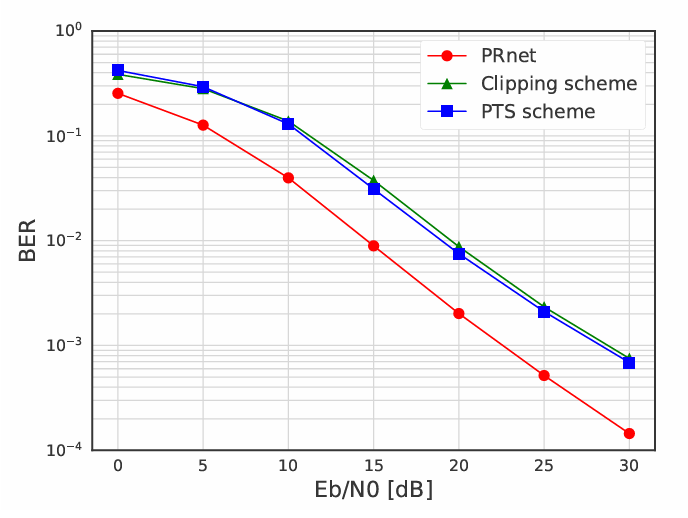
\includegraphics[width=\textwidth]{Figures/PRNet/prnet_ber.png}
        \caption{Original paper's evaluation~\cite{kim2017novel}}
        \label{fig:prnet_ber_paper_explanation}
    \end{subfigure}
    \hfill
    \begin{subfigure}[b]{0.48\textwidth}
        
\includegraphics[width=\textwidth]{Figures/PRNet/PRNet - Results/ber_vs_snr_rayleigh.jpg}
        \caption{Reproduced via our implementation}
        \label{fig:prnet_ber_reproduced_explanation}
    \end{subfigure}
    \caption{BER vs.\ SNR comparison of conventional PAPR reduction schemes and PRNet. Both the (a) original paper and (b) our reproduction demonstrate that PRNet achieves the lowest BER among the plotted schemes because the decoder is trained jointly with the encoder to invert the learned constellation shaping.}
    \label{fig:prnet_ber}
\end{figure}

Several observations are worth highlighting:

\begin{itemize}
    \item \textbf{Clipping} reduces PAPR but introduces in-band distortion, so its BER is degraded, especially at high SNR where the clipping noise becomes the dominant error source.
    \item \textbf{PTS} is distortionless in principle, but it requires side information and multiple IFFT computations.
    \item \textbf{PRNet} achieves BER that is \emph{lower} than the plotted PAPR-reduction baselines.  This is possible because the encoder-decoder pair is trained jointly: the encoder shapes the constellation in a way that the decoder can exploit, effectively learning an implicit coding gain under the simulated channel~\cite{kim2017novel}.
\end{itemize}

\begin{keyinsight}[Why PRNet's BER Is Lower Than Conventional OFDM]
    This result often surprises first-time readers: how can a PAPR-reduction method avoid the BER penalty usually seen with clipping?  The explanation is that the encoder does not merely apply phase rotations (like SLM) --- it completely reshapes the constellation geometry.  The jointly trained decoder is specifically designed to decode this custom geometry, giving it an advantage over a receiver that treats the shaping as distortion.  In effect, the autoencoder has learned a form of \emph{joint source-channel coding} that is optimised for the specific channel conditions it was trained on~\cite{kim2017novel}.
\end{keyinsight}


\subsection{PAPR Reduction (Paper Figure~3)}

The CCDF plot below shows the probability that the PAPR of a randomly generated OFDM symbol exceeds a given threshold.
\begin{keyinsight}[Reading the CCDF at $10^{-3}$]
    The most standard way to read PAPR performance from a CCDF plot is to pick a fixed probability level --- commonly $10^{-3}$ (meaning ``1 in 1000 symbols'') --- and read off the PAPR value on the $x$-axis. In the paper's plotted Fig.~3, conventional OFDM is around 10--11~dB at $\mathrm{CCDF} = 10^{-3}$, while the red PRNet curve is near 3~dB.  That visual result matches the paper's textual claim that $\mathrm{Prob}\{\mathrm{PAPR}>3~\mathrm{dB}\}<0.1\%$~\cite{kim2017novel}.
\end{keyinsight}

The PRNet curve is shifted \emph{significantly} to the left compared to conventional OFDM.  The paper reports that with PRNet, the probability of PAPR exceeding 3~dB is less than 0.1\%~\cite{kim2017novel}.  In practical terms, this means the High-Power Amplifier at the transmitter can operate with substantially less Input Back-Off, directly improving power efficiency.

\begin{misconception}
    \textbf{``The paper's red CCDF curve is standard physical PAPR.''} \\
    A mathematical critique of the authors' open-source code (\url{https://github.com/gomman/OFDM_PAPR_reduction}) reveals a metric discrepancy: the CCDF is plotted using an amplitude-based proxy rather than the standard power-based definition. Specifically, their Python implementation computes the metric as:
    \begin{codelisting}[numbers=none]{Authors' Proxy Metric Implementation}{Python}
        papr_proxy = 10 * np.log10(np.max(np.abs(x_norm)))
    \end{codelisting}
    which corresponds mathematically to:
    \begin{equation*}
        \mathrm{PAPR}_{\mathrm{proxy}}\,\mathrm{[dB]} = 10\log_{10}\left(\max_{n} \lvert x_{\mathrm{norm}}[n] \rvert\right),
    \end{equation*}
    where $x_{\mathrm{norm}}[n]$ represents the time-domain symbol normalized to unit average power. In contrast, the standard physical PAPR (in dB) is a power ratio computed as:
    \begin{codelisting}[numbers=none]{Standard Physical Power Metric}{Python}
        papr_standard = 10 * np.log10(np.max(np.abs(x_norm)**2))
    \end{codelisting}
    which corresponds to:
    \begin{equation*}
        \mathrm{PAPR}_{\mathrm{standard}}\,\mathrm{[dB]} = 10\log_{10}\left(\max_{n} \lvert x_{\mathrm{norm}}[n] \rvert^2\right) = 20\log_{10}\left(\max_{n} \lvert x_{\mathrm{norm}}[n] \rvert\right).
    \end{equation*}
    Consequently, the proxy metric is mathematically exactly half of the standard physical PAPR in decibels:
    \begin{equation*}
        \mathrm{PAPR}_{\mathrm{standard}}\,\mathrm{[dB]} = 2 \cdot \mathrm{PAPR}_{\mathrm{proxy}}\,\mathrm{[dB]}.
    \end{equation*}
    Evaluating the trained model under the standard power metric yields a physical PAPR of approximately 6~dB at a CCDF of $10^{-3}$, which still represents a significant 4--5~dB reduction from the conventional OFDM baseline (typically 10--11~dB) but is less extreme than the 3~dB reported in the paper's figures.

    Figure~\ref{fig:prnet_ccdf} reproduces these results by plotting both the standard metric and the proxy metric on the same axis alongside the paper's original graph.

    \begin{figure}[H]
        \centering
        \begin{subfigure}[b]{0.48\textwidth}
            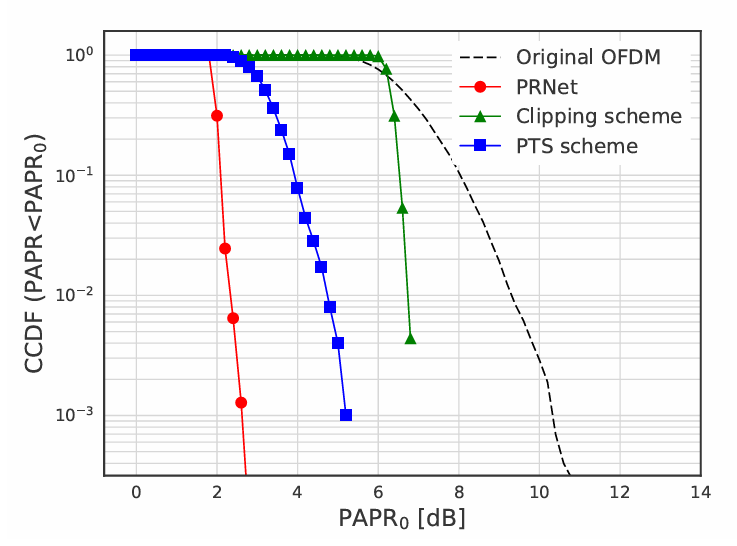
\includegraphics[width=\textwidth]{Figures/PRNet/prnet_ccdf.png}
            \caption{Original paper's evaluation~\cite{kim2017novel}}
            \label{fig:prnet_ccdf_paper_explanation}
        \end{subfigure}
        \hfill
        \begin{subfigure}[b]{0.48\textwidth}
            
\includegraphics[width=\textwidth]{Figures/PRNet/PRNet - Results/ccdf_papr_rayleigh.jpg}
            \caption{Reproduced via our implementation}
            \label{fig:prnet_ccdf_reproduced_explanation}
        \end{subfigure}
        \caption{CCDF of PAPR comparison. (a) The original paper reports a curve reaching 3~dB. (b) Our reproduction plots both the standard physical PAPR metric and the authors' amplitude proxy metric. The 3~dB curve matches the paper's reported performance due to the proxy metric, while the standard physical metric yields a realistic 6~dB PAPR.}
        \label{fig:prnet_ccdf}
    \end{figure}
\end{misconception}


\subsection{Optimal Corruption Level (Paper Figure~4)}

The BER-versus-corruption curves below show the BER of PRNet models trained at different corruption levels $\eta$, validating the two-stage training procedure.

\begin{figure}[H]
    \centering
    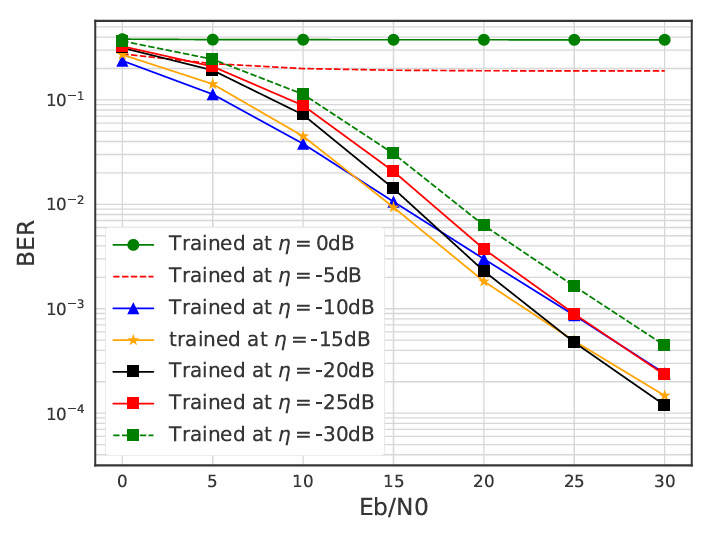
\includegraphics[width=0.55\linewidth]{Figures/PRNet/prnet_ber_corruption.png}
    \caption{BER of PRNet trained at different corruption levels $\eta$. The curve for $\eta = -15$~dB consistently yields the lowest BER across the entire SNR range. Reproduced from~\cite{kim2017novel}.}
    \label{fig:prnet_ber_corruption}
\end{figure}

The results confirm the training intuition developed above:

\begin{itemize}
    \item \textbf{$\eta = -30$~dB (too little noise):} The decoder learned very tight decision boundaries during training and cannot handle the larger noise encountered at test time. BER is poor across all SNR values.

    \item \textbf{$\eta = 0$~dB (too much noise):} The noise during training was so severe that the decoder could not learn meaningful decision boundaries at all.  BER is also poor.

    \item \textbf{$\eta = -15$~dB (the sweet spot):} The noise was strong enough to force the decoder to learn robust boundaries, but gentle enough that the constellation points remained distinguishable. This $\eta$ yields the lowest BER across \emph{all} tested SNR values, validating the paper's choice of $\eta^\star = -15$~dB~\cite{kim2017novel}.
\end{itemize}


\subsection{The BER--PAPR Trade-off via \texorpdfstring{$\lambda$}{lambda} (Paper Figure~5)}

The trade-off curves below show how varying $\lambda$ affects both BER and average PAPR at a fixed SNR of 20~dB.

\begin{figure}[H]
    \centering
    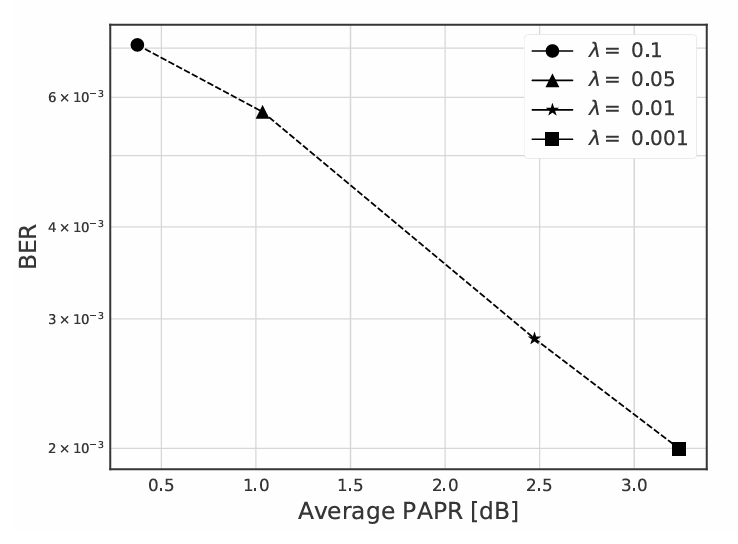
\includegraphics[width=0.55\linewidth]{Figures/PRNet/prnet_ber_papr_lambda.png}
    \caption{BER vs.\ average PAPR by varying $\lambda$ when SNR $= 20$~dB. Larger $\lambda$ reduces PAPR but increases BER, confirming the fundamental trade-off. Reproduced from~\cite{kim2017novel}.}
    \label{fig:prnet_ber_lambda}
\end{figure}

The results visualise the trade-off that $\lambda$ controls:

\begin{itemize}
    \item As $\lambda$ increases from 0 to 0.1, the average PAPR decreases monotonically --- the encoder sacrifices more constellation clarity for peak suppression.
    \item Simultaneously, BER increases --- the decoder's reconstruction task becomes harder because the constellation is increasingly distorted.
    \item At $\lambda = 0.01$, the paper reports a practical sweet spot: meaningful PAPR reduction while keeping BER competitive with the conventional PAPR-reduction baselines~\cite{kim2017novel}.
\end{itemize}


\subsection{Computational Overhead}

At inference time, PRNet replaces the $U$-fold \emph{search} of SLM/PTS with a single forward pass through two DNNs plus one IFFT/FFT pair.
The original paper reports the computational complexity of this forward pass as~\cite{kim2017novel}:
\begin{equation*}
    \mathcal{C}_{\mathrm{DNN\_paper}}
    = \mathcal{O}(L \cdot K \cdot M),
\end{equation*}
where $L$ is the number of hidden layers, $K = 2048$ is the number of hidden nodes per layer, and $M$ is the input modulation order.

\begin{misconception}
    \textbf{``The complexity of a fully connected neural network depends linearly on the hidden layer width.''} \\
    This is a typographical error in the paper's formal complexity statement. A standard complexity analysis of a fully connected neural network indicates that the linear transformation at each hidden layer requires a matrix-vector multiplication of size $K \times K$. Thus, the hidden layer computations dominate, yielding a true per-pass complexity of:
    \begin{equation*}
        \mathcal{C}_{\mathrm{DNN\_true}} = \mathcal{O}(L \cdot K^2),
    \end{equation*}
    or specifically, $L \cdot K^2 + d_{\mathrm{in}} K + d_{\mathrm{out}} K$ operations, which is independent of the input modulation order $M$ for large $K$. Despite this typo, the inference cost remains fixed and independent of the candidate search space $U$ required by scrambling methods.
\end{misconception}

Kim et al.\ report measured execution times~\cite{kim2017novel}:

\begin{table}[H]
    \centering
    \caption{Comparison of execution times for different PAPR reduction methods~\cite{kim2017novel}.}
    \label{tab:prnet_timing}
    \begin{tabular}{@{} l r @{}}
        \toprule
        \textbf{Method}             & \textbf{Execution time ($\mu$s)} \\
        \midrule
        PTS                         & 2{,}890                          \\
        Clipping and filtering      & 1{,}415                          \\
        PRNet (without parallelism) & 2{,}304                          \\
        PRNet (with GPU)            & 480                              \\
        \bottomrule
    \end{tabular}
\end{table}

With GPU-based parallel computation, PRNet is approximately \textbf{6 times faster} than PTS and \textbf{3 times faster} than clipping and filtering, while simultaneously achieving better BER and PAPR performance.  Even without parallelism, PRNet is comparable in speed to PTS while being fundamentally simpler --- it has no search loop, no candidate comparison, and no side information.

In short, the simulation results show that PRNet can learn a low-PAPR, decodable constellation mapping without side information.  The paper reports a dramatic PRNet CCDF shift; our code audit indicates that the published red curve corresponds to a peak-amplitude proxy, while standard power-PAPR evaluation still shows a meaningful but less extreme reduction.  The two-stage training procedure identifies $\eta^\star = -15$~dB as the best corruption level in the paper's setting, and $\lambda = 0.01$ as its selected BER--PAPR trade-off.  Computationally, the single forward pass is faster than the multi-IFFT search of SLM/PTS when GPU acceleration is used.


% ============================================================================
\section{Common Misconceptions}
% ============================================================================

\begin{misconception}
    \textbf{``Once trained, PRNet works for any $N$ and modulation.''} \\
    The encoder and decoder dimensions are fixed by the chosen representation. In the paper's one-hot formulation, the network input/output dimension is $NM$ and the encoder's physical signal output is $2N$; in our coordinate-based reproduction, the network input/output dimension is $2N$.  Either way, a PRNet trained for $N = 64$ subcarriers with QPSK cannot be directly used for $N = 128$ or for 16-QAM, because the weight matrices and learned signal statistics no longer match.  Changing $N$ or $M$ requires a new architecture or at least substantial retraining.
\end{misconception}

\begin{misconception}
    \textbf{``The AWGN-trained model will work on a Rayleigh channel.''} \\
    The decoder learns an inverse mapping that is specific to the channel statistics it was trained on.  If the model is trained with AWGN noise only and then deployed on a Rayleigh fading channel --- where the signal is randomly attenuated and rotated by complex fading coefficients --- the decoder will fail because it has never encountered that kind of distortion.  The constellation shapes that are ``safe'' under AWGN may not be safe under fading, and the decoder's decision boundaries are calibrated for a noise distribution it has never seen.  The CCDF may still look similar because PAPR is measured before the channel, but the BER can degrade sharply.  Retraining or fine-tuning under the target channel model is required when the channel statistics change.
\end{misconception}

\begin{misconception}
    \textbf{``PRNet learns QPSK symbols and rotates them.''} \\
    PRNet does not start with QPSK points and apply phase rotations (that would be SLM).  Instead, the encoder takes the raw bit sequence and directly computes entirely new complex numbers from scratch.  These numbers are not constrained to any standard constellation grid --- they are continuous-valued coordinates in the complex plane, shaped specifically for the current bit pattern.  There are no ``base QPSK points'' being modified; the encoder invents its own constellation geometry from the ground up~\cite{kim2017novel}.
\end{misconception}


% ============================================================================
\section{Limitations and Open Problems}
% ============================================================================

PRNet is a foundational result, but several limitations remain (from the paper's discussion and our own implementation experience):

\begin{enumerate}
    \item The fully connected architecture scales quadratically with the number of subcarriers. The first encoder layer has $d_{\mathrm{in}} \times K = 2N \times 2048$ weights. For $N = 64$, this requires $128 \times 2048 = 262{,}144$ parameters in the input layer alone. Scaling to standard practical systems with $N = 1024$ or $N = 2048$ subcarriers leads to parameter explosion and prohibitive memory overhead, indicating that fully connected topologies cannot scale to practical systems without transitioning to convolutional, attention, or signal-unfolding architectures~\cite{kim2017novel}.
    \item \textbf{Channel mismatch:} The paper models a Rayleigh fading channel, and the network's performance is tightly coupled to how well the training channel matches the actual deployment environment.  Extending PRNet to clearly specified frequency-selective channels, imperfect channel state information (CSI), pilot overhead, and rapidly time-varying scenarios remains an open problem~\cite{kim2017novel}.
    \item \textbf{Retraining across configurations:} Any change in system parameters --- modulation order ($M$), number of subcarriers ($N$), pilot structure, coding rate --- changes the dimensionality or statistical properties of the signal. If the dimensions change, the architecture must change as well; if only the channel or operating point changes, fine-tuning may be possible, but a fresh validation campaign is still required.
    \item \textbf{PAPR metric ambiguity:} The paper defines CCDF in terms of PAPR, but the released PRNet code plots a peak-amplitude proxy for the PRNet CCDF.  This does not invalidate the learned approach, but it means the most dramatic Fig.~3 number should be interpreted carefully and standard power-PAPR results should be reported separately.
    \item \textbf{Interpretability:} PRNet learns an implicit constellation shaping rule that is encoded in millions of weight values.  Understanding \emph{what} specific shaping the network has learned --- for instance, whether it has discovered a structure analogous to a known coding scheme --- is extremely difficult.  This makes it hard to diagnose failures or to prove guarantees about the system's worst-case behaviour, unlike explicit methods like SLM where the phase rotation rule is transparent.
\end{enumerate}


% ============================================================================
\section{Connection to Other Approaches}
% ============================================================================

PRNet established the autoencoder paradigm for PAPR reduction.  Subsequent works build on Kim's core insight --- treat the communication chain as an end-to-end trainable system and include PAPR explicitly in the learning objective --- while addressing one or more of PRNet's limitations:

\begin{itemize}
    \item \textbf{Hao et al.\ (2019)} explicitly connect the autoencoder to the SLM framework by constraining the encoder to learn \emph{phase factors} rather than an unconstrained nonlinear mapping.  This retains SLM's interpretability while gaining the autoencoder's ability to optimise phase sequences via gradient descent.
    \item \textbf{Alnaseri et al.\ (2025)} transfer the autoencoder idea to coherent optical OFDM (CO-OFDM), incorporating fibre-channel effects such as chromatic dispersion and Kerr nonlinearity into the end-to-end training pipeline.
    \item \textbf{Zou et al.\ (2021)} use a related DNN architecture within a signal-cancellation framework rather than a pure autoencoder, adding a dedicated peak-cancellation and signal-recovery module that achieves PAPR reduction without requiring a jointly trained decoder.
\end{itemize}

In short, PRNet was the first to demonstrate that deep learning can jointly optimise BER and PAPR in OFDM.  Its limitations --- scalability, channel sensitivity, and interpretability --- define the natural research agenda that subsequent works address.
